% standalone wrapper for a tikz picture
\documentclass[tikz,border=2pt]{standalone}
\usepackage{xcolor}
\usepackage{tikz}
\usepackage{pgfplots}
\pgfplotsset{compat=1.18}
\usetikzlibrary{shapes,arrows,positioning,shadows,patterns,arrows.meta,calc}
\definecolor{cwAlert}{RGB}{220,50,50}
\definecolor{cwFlow}{RGB}{50,120,220}
\definecolor{cwDecoy}{RGB}{120,180,50}
\definecolor{cwBorder}{RGB}{80,80,80}
\definecolor{ImperialBlue}{RGB}{0,62,116}
\definecolor{ImperialNavy}{RGB}{0,33,71}
\definecolor{ImperialLightBlue}{RGB}{155,203,235}
\begin{document}

% Standalone axis-only figure (no surrounding center/tikz nesting)
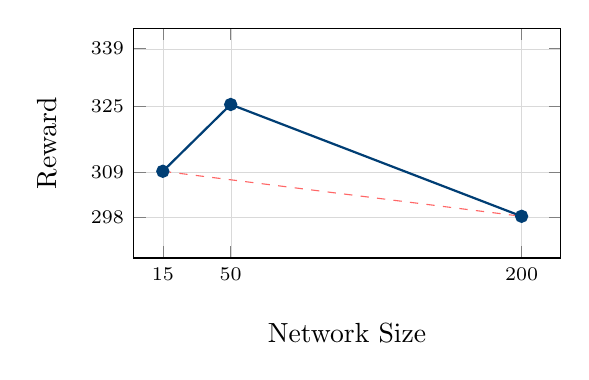
\begin{tikzpicture}
\begin{axis}[
    width=7cm,
    height=4.5cm,
    xlabel={Network Size},
    ylabel={Reward},
    xlabel style={yshift=-0.3cm},
    ylabel style={yshift=0.2cm},
    xmin=0, xmax=220,
    ymin=288, ymax=344,
    xtick={15,50,200},
    xticklabel style={font=\scriptsize},
    ytick={298,309,325,339},
    yticklabel style={font=\scriptsize},
    grid=major,
    grid style={line width=.1pt, draw=gray!30},
    axis background/.style={fill=white},
]
\addplot[thick, draw=ImperialBlue, mark=*, mark options={fill=ImperialBlue}] coordinates {
    (15,309.14)
    (50,325.42)
    (200,298.17)
};
\addplot[dashed, red!60] coordinates {(15,309.14) (200,298.17)};
\end{axis}
\end{tikzpicture}

\end{document}
